\documentclass[a4paper,11pt]{memoir}

\ifpdf
\usepackage[utf8]{inputenc}
\usepackage[T1]{fontenc}
\fi

%\usepackage{german}
%\usepackage[english]{babel}
%\usepackage[german]{translator}
%\usepackage{hyperref}

\usepackage{import}
\usepackage{xifthen}
%\usepackage{pdfpages}
\usepackage{transparent}
\usepackage{subfig}
\usepackage{hhline}

\newcommand{\incfig}[1]{%
	\def\svgwidth{\columnwidth}
	\import{./bilder/}{#1.pdf_tex}
}

% This is the only file needed for actually using the smart-thesis style.
%
% Smart Thesis LaTeX template
%
% [To underline the amateurish flavour of this template, let's start with some
% nifty ASCII-Art (http://www.network-science.de/ascii/)...]
%
%      #######
%    /       ###
%   /         ##                                          #
%   ##        #                                          ##
%    ###                                                 ##
%   ## ###      ### /### /###     /###   ###  /###     ########
%    ### ###     ##/ ###/ /##  / / ###  / ###/ #### / ########
%      ### ###    ##  ###/ ###/ /   ###/   ##   ###/     ##
%        ### /##  ##   ##   ## ##    ##    ##            ##
%          #/ /## ##   ##   ## ##    ##    ##            ##
%           #/ ## ##   ##   ## ##    ##    ##            ##
%            # /  ##   ##   ## ##    ##    ##            ##
%  /##        /   ##   ##   ## ##    /#    ##            ##
% /  ########/    ###  ###  ### ####/ ##   ###           ##
%/     #####       ###  ###  ### ###   ##   ###           ##
%|
% \)
%
%
%  /###           /  /
% /  ############/ #/                              #
%/     #########   ##                             ###
%#     /  #        ##                              #
% ##  /  ##        ##
%    /  ###        ##  /##      /##       /###   ###        /###
%   ##   ##        ## / ###    / ###     / #### / ###      / #### /
%   ##   ##        ##/   ###  /   ###   ##  ###/   ##     ##  ###/
%   ##   ##        ##     ## ##    ### ####        ##    ####
%   ##   ##        ##     ## ########    ###       ##      ###
%    ##  ##        ##     ## #######       ###     ##        ###
%     ## #      /  ##     ## ##              ###   ##          ###
%      ###     /   ##     ## ####    /  /###  ##   ##     /###  ##
%       ######/    ##     ##  ######/  / #### /    ### / / #### /
%         ###       ##    ##   #####      ###/      ##/     ###/
%                         /
%                        /
%                       /
%                      /
%
% About:
% ======
%
% This template is a re-implementation of the "classicthesis" template by André
% Miede. However, it uses the "memoir" class as a basis, eliminating most
% of the external packages required by "classicthesis" and thus (hopefully)
% achieving a higher compatibility with other LaTeX packages. Large parts of
% the code have been adapted (ransacked) from André Miedes code.
%
% You can find more information about "classicthesis" at CTAN:
%
% https://www.ctan.org/pkg/classicthesis
%
% More information about the "memoir" package can be found here:
%
% https://www.ctan.org/pkg/memoir
%
%
% Authors:
% ========
%
% Jan Philip Göpfert, Andreas Stöckel
%
%
% License:
% ========
%
% This LaTeX template is published under the Creative Commons Zero license. To
% the extent possible under law, the authors have waived all copyright and
% related neighboring rights to Smart Thesis. This work is published from:
% Germany.
%


%
% EXTERNAL PACKAGES
%
\usepackage[usenames,dvipsnames,svgnames]{xcolor}
\usepackage{ragged2e} % for marginnote

%\usepackage{listings}

%
% FONT DEFINITIONS
%

% Use the following code for XeLaTeX
\ifxetex

% Setup microtype for XeLaTeX
\usepackage[expansion=false,final]{microtype}

% Load the texgyrepagella font as main font and set the ``mathpazo'' font as
% math font
\usepackage{fontspec}
\usepackage{mathpazo}
\setmainfont%
	[%
		BoldFont       = texgyrepagella-bold.otf,
		ItalicFont     = texgyrepagella-italic.otf,
		BoldItalicFont = texgyrepagella-bolditalic.otf,
		Ligatures      = TeX
	]%
	{texgyrepagella-regular.otf}

% Define a new 'widespaced' font that is used in section headings
% or chapter titles. For backwards compatibility reasons this uses
% the old calling convention \newfontfamily\fontname[<options>{font}
% instead of the newer \newfontfamily\fontname{font}[<options>]
\newfontfamily\widespaced[%
	LetterSpace=15,%
	WordSpace={1.25, 1.25, 1.25}%
]{texgyrepagella-regular.otf}%

\DeclareRobustCommand{\spacedallcaps}[1]{%
	{\widespaced\oldstylenums{\MakeTextUppercase{#1}}}%
}%
\DeclareRobustCommand{\spacedlowsmallcaps}[1]{%
	{\widespaced\oldstylenums{\textsc{\MakeTextLowercase{#1}}}}%
}%
\fi

% Use the following code for pdfLaTex
\ifpdf

% Setup microtype for pdfLaTex
\usepackage[final,tracking=true,kerning=true,spacing=nonfrench]{microtype}


\usepackage[sc]{mathpazo}

\DeclareRobustCommand{\spacedallcaps}[1]{\textls[160]{\oldstylenums{\textsc{\MakeTextUppercase{#1}}}}}%
\DeclareRobustCommand{\spacedlowsmallcaps}[1]{\textls[80]{\oldstylenums{\textsc{\MakeTextLowercase{#1}}}}}%
\fi

% Increase linespread for Palatino
\renewcommand{\linespread}{1.05}

%
% COLOR DEFINITIONS
%

\definecolor{smartgray}{gray}{0.55}
\definecolor{smartred}{HTML}{800000}
\definecolor{smartplum}{HTML}{47294F}
\definecolor{smartblue}{HTML}{193A6B}
\definecolor{smartorange}{HTML}{AA4C00}
\definecolor{smartgreen}{HTML}{3C7705}
\definecolor{smartbutter}{HTML}{A08300}

\definecolor{tangored}{HTML}{CC0000}
\definecolor{tangoplum}{HTML}{75507B}
\definecolor{tangoblue}{HTML}{3465A4}
\definecolor{tangoorange}{HTML}{F57900}
\definecolor{tangogreen}{HTML}{73D216}
\definecolor{tangobutter}{HTML}{EDD400}

\definecolor{shadecolor}{gray}{0.95}

\colorlet{heading}{smartgray}
\colorlet{ref}{smartblue}
\colorlet{cite}{smartgreen}
\colorlet{url}{smartred}
\colorlet{caption}{black}
\colorlet{margincaption}{caption}

%
% SECTIONING STYLES (toledo)
%

% See http://tex.stackexchange.com/questions/161577/memoir-hangnum-chapter-number-in-right-margin-switch for the inspiration

\setsecnumdepth{subsection}

\makeatletter
\makechapterstyle{toledo}{%
	\chapterstyle{default}

	\renewcommand*{\chapterheadstart}{\vspace*{0.0cm}}

	\renewcommand*{\chapnumfont}{\normalfont\color{heading}\addfontfeature{SizeFeatures={Size=110}}}
	\newfont{\chapterNumber}{eurb10 scaled 7000}
	\renewcommand*{\chapnumfont}{\chapterNumber\color{heading}}
	\renewcommand*{\printchaptername}{}
	\renewcommand*{\chapternamenum}{}
	\renewcommand*{\printchapternum}{%
		\raisebox{0pt}[0pt][0pt]{%
		\makebox[0pt][l]{%
		\makebox[\dimexpr\textwidth+5.45em\relax][l]{%
			\parbox[t]{\textwidth}{\mbox{}}%
			\parbox[t]{5.45em}{\hfill\chapnumfont \thechapter}}}}}%
	\renewcommand*{\chapternamenum}{}
	\renewcommand*{\afterchapternum}{}

	\renewcommand*{\afterchaptertitle}{%
	\par\parbox{\textwidth}{\hrulefill}\par%
	\vspace*{4ex}}
	\renewcommand*{\chaptitlefont}{\normalfont\large}
	\renewcommand*{\printchaptertitle}[1]{%
		\parbox[b]{\textwidth}{%
			\raggedright\chaptitlefont\spacedallcaps{##1}%
		}%
	}

	\setsecheadstyle{\spacedlowsmallcaps}
	\setsecindent{-3.5ex}
	\setbeforesecskip{-4ex plus -1ex minus -.2ex}
	\setaftersecskip{4ex plus 1ex minus .2ex}

	\setsubsecheadstyle{\itshape}
	\setbeforesubsecskip{-4ex plus -1ex minus -.2ex}
	\setaftersubsecskip{4ex plus 1ex minus .2ex}
	\setsecnumformat{\spacedlowsmallcaps{\csname the##1\endcsname\quad}}

%	\setparaheadstyle{\normalsize\itshape}

	\renewcommand*{\abstractnamefont}{\spacedlowsmallcaps}
}
\makeatother

\chapterstyle{toledo}

%
% FIGURES
%

\captionstyle{\small}
\captionnamefont{\slshape\color{caption}}

\newsubfloat{figure}% Create subfloat in figure environment
\newsubfloat{table}% Create subfloat in table environment

%
% ACKNOWLEDGEMENT
%

\makeatletter
\newcommand{\acknowledgementname}{Acknowledgements}
\newenvironment{acknowledgement}{%
  \setup@bstract
  \if@bsrunin\else
    \ifnumber@bs \num@bs \else
      \begin{\absnamepos}\abstractnamefont\acknowledgementname\end\absnamepos%
      \vspace{\abstitleskip}%
    \fi
  \fi
  \put@bsintoc%
  \begin{@bstr@ctlist}\if@bsrunin\@bsrunintitle\fi\abstracttextfont}%
  {\par\end{@bstr@ctlist}}

\newcommand{\smartcopyright}[1]{\begingroup%
	\pagebreak%
	\thispagestyle{empty}%
	\footnotesize%
	\par\vspace*{\fill}%
	\hspace{-1.1cm}%
	\parbox{10cm}{%
		\noindent%
		Copyright \textcopyright\ \the\year\ \applytolist[, ]{}{\@author}\\[0.5cm]%
		{#1}%
	}%
\endgroup}

\newcommand{\smartinitialepigraph}[2]{\begingroup
	\cleardoublepage
	\thispagestyle{empty}
	\vspace*{2cm}
	\epigraph{#1}{#2}
	\cleardoublepage
\endgroup}

\let\oldepigraph\epigraph
\renewcommand{\epigraph}[2]{\oldepigraph{#1}{\spacedlowsmallcaps{#2}}}

\makeatother

%
% MARGINNOTE
%

%
% There are three commands for placing elements in the margin:
%
% \marginnote{<TEXT>}
% Just like \marginpar but with correct formating
%
% \marginfig{<SHORT CAPTION>}{<FIGURE CONTENT>}{<LONG CAPTION>}{\label{<LABEL>}}
% \margintbl{<SHORT CAPTION>}{<TABLE CONTENT>}{<LONG CAPTION>}{\label{<LABEL>}}
% Places a figure/table in the margin
% - <SHORT CAPTION> is the caption as it occurs in the list of figures/tables
% - <FIGURE CONTENT>/<TABLE CONTENT> is the actual figure/table content
% - <LONG CAPTION> is the caption below the figure
% - <LABEL> is the label -- we decided to let you explicitly type "\label" here
% as this allows LaTeX editors to index the label and provide auto completion.
%

% Define the "marginnote" command. For compatibility reasons
% we do not override marginpar.
\strictpagecheck
\newcommand{\marginnote}[1]{\hspace*{0pt}\marginpar{
	\microtypesetup{disable}%
	\slshape\footnotesize%
	\vspace*{-0.725em}%
	\checkoddpage%
	\ifoddpage%
		\RaggedRight%
	\else%
		\RaggedLeft%
	\fi%
	{#1}%
	\microtypesetup{enable}%
}\ignorespaces}

\newcommand{\marginfloat}[8]{\marginnote{{#1}%
\par\refstepcounter{#4}\textcolor{margincaption}{#5 #6}: {#2}#3}%
\addcontentsline{#7}{#4}{\protect\numberline {#6}{\ignorespaces #8}}\ignorespaces}

\newcommand{\marginfig}[4]{\marginfloat{#2}{#3}{#4}{figure}{Figure}{\thefigure}{lof}{#1}}
\newcommand{\margintbl}[4]{\marginfloat{#2}{#3}{#4}{table}{Table}{\thetable}{lot}{#1}}

%
% PAGE STYLE (headers, footers)
%

\makeatletter

% Deactivate capitalization of headers.
\nouppercaseheads

% Define the new "berlin" style.
\makepagestyle{berlin}

% Display the page number in the footer.
\makeevenfoot{berlin}{\thepage}{}{}
\makeoddfoot{berlin}{}{}{\thepage}

% Override the chapter style with the unfinished "berlin" style
% to eliminate the header and to make sure a consistent footer
% style is used.
\copypagestyle{chapter}{berlin}

% Define the "berlin" style
\makepsmarks{berlin}{%
	\def\chaptermark##1{%
	\markboth{\memUChead{%
		\ifnum \c@secnumdepth >\m@ne
		\if@mainmatter
			\@chapapp\ \thechapter. \ %
		\fi
		\fi
		##1}}{}}%
	\def\tocmark{\markboth{\memUChead{\contentsname}}{\memUChead{\contentsname}}}%
	\def\lofmark{\markboth{\memUChead{\listfigurename}}{\memUChead{\listfigurename}}}%
	\def\lotmark{\markboth{\memUChead{\listtablename}}{\memUChead{\listtablename}}}%
	\def\bibmark{\markboth{\memUChead{\bibname}}{\memUChead{\bibname}}}%
	\def\indexmark{\markboth{\memUChead{\indexname}}{\memUChead{\indexname}}}%
	\def\sectionmark##1{%
	\markright{\memUChead{%
		\ifnum \c@secnumdepth > \z@
		\thesection. \ %
		\fi %
		##1}}}}
\makepsmarks{berlin}{%
	\createmark{chapter}{left}{nonumber}{}{}
	\createmark{section}{right}{shownumber}{}{\ }
	\createplainmark{toc}{both}{\contentsname}
	\createplainmark{lof}{both}{\listfigurename}
	\createplainmark{lot}{both}{\listtablename}
	\createplainmark{bib}{both}{\bibname}
	\createplainmark{index}{both}{\indexname}
	\createplainmark{glossary}{both}{\glossaryname}
}

% Discriminate between "oneside" and "twoside" documents.
\if@twoside
	\makeevenhead{berlin}{\spacedlowsmallcaps{\leftmark}}{}{}
	\makeoddhead{berlin}{}{}{\spacedlowsmallcaps{\rightmark}}
\else
	\makeoddhead{berlin}{\spacedlowsmallcaps{\rightmark}}{}{}
\fi

% Use the berlin style.
\pagestyle{berlin}

\makeatother

%
% FOOTNOTES
%

\footmarkstyle{\textsc{#1}}
\setlength{\footmarkwidth}{-0.5em}
\setlength{\footmarksep}{0.5em}
\setlength{\footparindent}{0em}

%
% EPIGRAPHS
%
\makeatletter

% Make the epigraph span two third of the text width
\setlength{\epigraphwidth}{0.66\textwidth}

% Disable the rule below the epigraph
\setlength{\epigraphrule}{0pt}

% Use the normal font size
\epigraphfontsize{\normalsize}

% Style the epigraph itself -- use italic text and
% flush it to the right
\newenvironment{epigraphstyle}{
%	\microtypesetup{disable}%
	\small\slshape%
%	\RaggedLeft%
}{%
%	\microtypesetup{enable}%
}
\epigraphtextposition{epigraphstyle}

% Style the epigraph source -- prepend it with a em-dash
% and make sure no indentation is added after the epigraph
\newenvironment{epigraphsourcestyle}%
{%#
	--- \small\raggedleft\color{smartred}%
}{%
	\@afterindentfalse\@afterheading%
}
\epigraphsourceposition{epigraphsourcestyle}

\makeatother

%
% TITLEPAGE
%

\makeatletter
\newcommand\thesistype[1]{\renewcommand\@thesistype{#1}}
\newcommand\@thesistype{}

\newcommand\discipline[1]{\renewcommand\@discipline{#1}}
\newcommand\@discipline{}

\newcommand\institution[1]{\renewcommand\@institution{#1}}
\newcommand\@institution{}

\newcommand\supervisors[1]{\renewcommand\@supervisors{#1}}
\newcommand\@supervisors{}

\newcommand\reviewers[1]{\renewcommand\@reviewers{#1}}
\newcommand\@reviewers{}

\newcommand\internalid[1]{\renewcommand\@internalid{#1}}
\newcommand\@internalid{}

\newcommand\subtitle[1]{\renewcommand\@subtitle{#1}}
\newcommand\@subtitle{}

\newcommand{\applytolist}[3][{,\\\vspace{0.1cm}}]{%
	\def\nextitem{\def\nextitem{#1}}%
	\@for \el:=#3\do{\nextitem{#2{\el}}}%
}

\newcommand{\smarttitle}{
{\begingroup
\thispagestyle{empty}
\makeatletter
\raggedright
\vfill
{\LARGE \spacedallcaps{\@thesistype} \\}
{\Large \spacedlowsmallcaps{\@discipline}\\}
\vfill
{\huge \textcolor{smartred}{\spacedallcaps{\@title}}\\}
\vspace{3mm}
{\LARGE \textcolor{smartred}{\spacedallcaps{\@subtitle}}\\}
\vfill
{\LARGE \applytolist{\spacedallcaps}{\@author}\\}
\vfill
{\Large \applytolist{\itshape}{\@institution}}
\vfill
{\Large \spacedlowsmallcaps{Reviewed by}\\}
\vspace{0.1cm}
{\large \applytolist{\spacedallcaps}{\@reviewers}}
\vfill
{\Large \spacedlowsmallcaps{Supervised by}\\}
\vspace{0.1cm}
{\large \applytolist{\spacedallcaps}{\@supervisors}}
\vfill
\vfill
{\Large \spacedlowsmallcaps{\today} \hfill \spacedlowsmallcaps{\@internalid}}
\vfill
\makeatother
\endgroup}}

\makeatletter
%
% PAGE LAYOUT
%
\settypeblocksize{23.45cm}{11.85cm}{*}
%\setlength{\textheight}{23.45cm}
%\setlength{\textwidth}{11.85cm}
\setlrmargins{3.141592653589793cm}{*}{*}
\setulmargins{*}{*}{*}
\setmarginnotes{0.8cm}{3.5cm}{1cm}
\checkandfixthelayout


% Contains some packages which are commonly used in a thesis.
% Note that these are optional.
\usepackage{csquotes} % Context sensitive quotation facilities. Recommended by babel and should be loaded before babel.

\usepackage[english]{babel} % Sets the language used. Essential for proper hyphenation. Translates key words like 'figure' or 'table'. Note that 'english' is American English.

\usepackage{latexsym,amsmath,amssymb,amsthm,amscd} % Provides math enviroments, math symbols and more things useful for math.

\usepackage{mathtools} % Enhances amsmath and provides further mathematical tools.

\usepackage{graphicx} % Provides inclusion of graphics and a proper interface for '\in­clude­graph­ics'.
% Su­per­sedes 'epsfig' and 'graphics'.

\usepackage{enumitem} % Provides control over list environments. Supersedes 'enumerate', which gives enumerate environment an optional argument which determines the style in which the counter is printed.

%\let\newfloat\undefined % Hack to make floatrow work with memoir.
%\usepackage{floatrow} % Handles alignment of floats (figures), with centering as default.

\usepackage{xspace} % Ugly hack that sometimes helps with otherwise missing spaces.

\usepackage[backgroundcolor=white,linecolor=smartblue,bordercolor=smartblue,textsize=footnotesize]{todonotes} % Todo notes.

% Use sans-serif font in todos to clearly distinguish it from other text
\makeatletter
\renewcommand{\todo}[2][]{\@bsphack\@todo[#1]{\sffamily{#2}}\@esphack\ignorespaces}
\makeatother

\usepackage[style=alphabetic,backend=biber]{biblatex} % Bibliography.

%\usepackage{algorithm} % Algorithms.
% Use default Memoir floats for algorithms
\newcommand{\algorithmname}{Algorithm}
\newcommand{\listalgorithmname}{List of Algorithms}
\newlistof{listofalgorithms}{loa}{\listalgorithmname}
\newfloat[chapter]{algorithm}{loa}{\algorithmname}
\newfixedcaption{\falgcaption}{algorithm}
\newlistentry[chapter]{algorithm}{loa}{0}
\cftsetindents{algorithm}{0em}{2.3em}
\makeatletter
\g@addto@macro\insertchapterspace{\addtocontents{loa}{\protect\addvspace{10pt}}}
\makeatother

%\usepackage{algpseudocode} % Algorithms.

\usepackage{varioref} % Automatically locates references on other pages. Load before hyperref.

%\usepackage[hidelinks]{hyperref} % Clickable references.
\usepackage[pdfencoding=auto,pdfborderstyle={/S/U/W 1},linkbordercolor=ref,colorlinks,linkcolor=ref,citecolor=cite,urlcolor=url]{hyperref} % Clickable references.

\usepackage[all]{hypcap} % Anchors links to the beginning of their respective floats. Load after hyperref.

\usepackage[noabbrev,capitalize,nameinlink]{cleveref} % Names references automatically. Load after hyperref.

\usepackage[toc,acronym]{glossaries} % Glossary.

\usepackage{booktabs}
\usepackage{multirow}

\usepackage{pgfplots}
\pgfplotsset{compat=1.8}
\pgfplotscreateplotcyclelist{smart}{%
  tangoplum,semithick,every mark/.append style={fill=tangoplum!80!black},mark=*\\%
  tangogreen,semithick,every mark/.append style={fill=tangogreen!80!black},mark=square*\\%
  tangoorange,semithick,every mark/.append style={fill=tangoorange!80!black},mark=otimes*\\%
  tangoblue,semithick,mark=star\\%
  tangobutter,semithick,every mark/.append style={fill=tangobutter!80!black},mark=diamond*\\%
  tangored,semithick,every mark/.append style={solid,fill=tangored!80!black},mark=*\\%
}
\pgfplotsset{cycle list name=smart}

\usepackage{listings}

\definecolor{mygreen}{rgb}{0,0.6,0}
\definecolor{mygray}{rgb}{0.5,0.5,0.5}
\definecolor{mymauve}{rgb}{0.58,0,0.82}

\lstset{ %
  backgroundcolor=\color{white},   % choose the background color; you must add \usepackage{color} or \usepackage{xcolor}
  basicstyle=\footnotesize,        % the size of the fonts that are used for the code
  breakatwhitespace=false,         % sets if automatic breaks should only happen at whitespace
  breaklines=true,                 % sets automatic line breaking
  captionpos=b,                    % sets the caption-position to bottom
  commentstyle=\color{mygreen},    % comment style
  deletekeywords={...},            % if you want to delete keywords from the given language
  escapeinside={\%*}{*)},          % if you want to add LaTeX within your code
  extendedchars=true,              % lets you use non-ASCII characters; for 8-bits encodings only, does not work with UTF-8
  frame=single,	                   % adds a frame around the code
  keepspaces=true,                 % keeps spaces in text, useful for keeping indentation of code (possibly needs columns=flexible)
  keywordstyle=\color{blue},       % keyword style
  language=C++,                	% the language of the code
  otherkeywords={*,...},           % if you want to add more keywords to the set
  numbers=left,                    % where to put the line-numbers; possible values are (none, left, right)
  numbersep=5pt,                   % how far the line-numbers are from the code
  numberstyle=\tiny\color{mygray}, % the style that is used for the line-numbers
  rulecolor=\color{black},         % if not set, the frame-color may be changed on line-breaks within not-black text (e.g. comments (green here))
  showspaces=false,                % show spaces everywhere adding particular underscores; it overrides 'showstringspaces'
  showstringspaces=false,          % underline spaces within strings only
  showtabs=false,                  % show tabs within strings adding particular underscores
  stepnumber=1,                    % the step between two line-numbers. If it's 1, each line will be numbered
  stringstyle=\color{mymauve},     % string literal style
  tabsize=2,	                   % sets default tabsize to 2 spaces
  title=\lstname,                   % show the filename of files included with \lstinputlisting; also try caption instead of title
  literate=%
    {Ö}{{\"O}}1
    {Ä}{{\"A}}1
    {Ü}{{\"U}}1
    {ß}{{\ss}}1
    {ü}{{\"u}}1
    {ä}{{\"a}}1
    {ö}{{\"o}}1
    {~}{{\textasciitilde}}1
}

\renewcommand{\lstlistingname}{Quellcode}


% Contains some macros which are commonly used in a thesis.
% Note that these are optional.
% Abbreviations
\newcommand*{\eg}{e.\,g.\@\xspace}
\newcommand*{\ie}{i.\,e.\@\xspace}
\newcommand*{\cf}{cf.\@\xspace}
\newcommand*{\etal}{et.\@ al.\@\xspace}
%\newcommand*{\etc}{etc.\@\xspace}
\makeatletter
\newcommand*{\etc}{%
  \@ifnextchar{.}%
    {etc}%
      {etc.\@\xspace}%
}
\makeatother

% Sets
\newcommand*{\R}{\mathbb{R}}
\newcommand*{\Q}{\mathbb{Q}}
\newcommand*{\Z}{\mathbb{Z}}
\newcommand*{\N}{\mathbb{N}}

% Matrix/vector operations
\newcommand*{\transpose}[1]{{#1^{\top}}}
\newcommand*{\inverse}[1]{{#1^{-1}}}
\newcommand*{\conjugate}[1]{{#1^{\ast}}}
\newcommand*{\pseudoinverse}[1]{{#1^{+}}}

% Stochastics
\newcommand*{\probability}[1]{{\mathrm{Pr}{#1}}}
\newcommand*{\expectation}[1]{{#1}}

% Optimization
\DeclareMathOperator*{\argmax}{arg\,max}
\DeclareMathOperator*{\argmin}{arg\,min}
\DeclareMathOperator{\lb}{lb}
\DeclareMathOperator{\sign}{sgn}

% These packages are only used in the demo and not necessarily
% required for smart-thesis.
\usepackage{todonotes}

% Loads bibliography for citations.
\addbibresource{thesis-bibliography.bib}


% Define all the metadata to be listed in \smarttitle and \smartcopyright
\thesistype{Master Thesis}
\discipline{Intelligent Systems}
\title{A configurable speech recognition pipeline for social robots}
\subtitle{Creating a Fusion Framework for analyzing speech data}
\author{Robert Feldhans}
\institution{University of Bielefeld,Technical Faculty, Central Lab Facilities}
\supervisors{Dr.-Ing.\@~Sven Wachsmuth,M.Sc.\@~Florian Lier,M.Sc.\@~Birte Carlmeyer}
\reviewers{Dr.-Ing.\@~Sven Wachsmuth,M.Sc.\@~Florian Lier}


\begin{document}

\frontmatter

\smarttitle

%!TEX root = thesis.tex

%=============================================================================


\chapter{Abstract}
- First introduction to speech recognition and related stuff

- then presentation of our pipeline, which is based on two pillars.

- Then evaluation based on two experiments to show the validity of this approach and performance of the proposed pipeline.

- Lastly we will discuss further work, improvements to the proposed pipeline, additional things to evaluate

\newpage

\tableofcontents

\mainmatter
%!TEX root = thesis.tex

\chapter{Introduction \& Motivation}
\label{motiv:start}
In order to be accepted by humans, social robots in general depend on \gls{hri} \cite{6926324}, which in turn is influenced and shaped by human-human interaction \cite{mediaequation}.
Since speech is one of the most important modalities of communication between humans, it is no surprise that it is also one of the most important parts of \gls{hri}.
In \gls{hri}, verbal dialogue can be divided into speech generation and the main interest of this thesis: speech understanding.

Being able to perfectly recognize the words a person spoke does not completely cover speech understanding, e.g. the perception and engagement of the speaker \cite{Ivaldi2017}.
An exemplary dialogue between a robot and two humans is depicted in a provided video\footnote{\url{https://www.youtube.com/watch?v=iEMKZdwJPE8}} and in stills in figure \ref{pic:moti:imustgonow}.
The video depicts parts of a RoboCup@home Task at the RoboCup World Championship 2018 in Montreal.
In three different instances two referees are giving a robot commands, but they take turns in speaking to the robot.
The robot does not recognize two different speakers, and thus, cannot react appropriately.
More so:
when asking for the confirmation of a specific command, it does not even seem to recognize that a different person gives this confirmation, or that the original referee walked away and no longer partakes in the conversation.

\begin{figure}[]
	\centering
	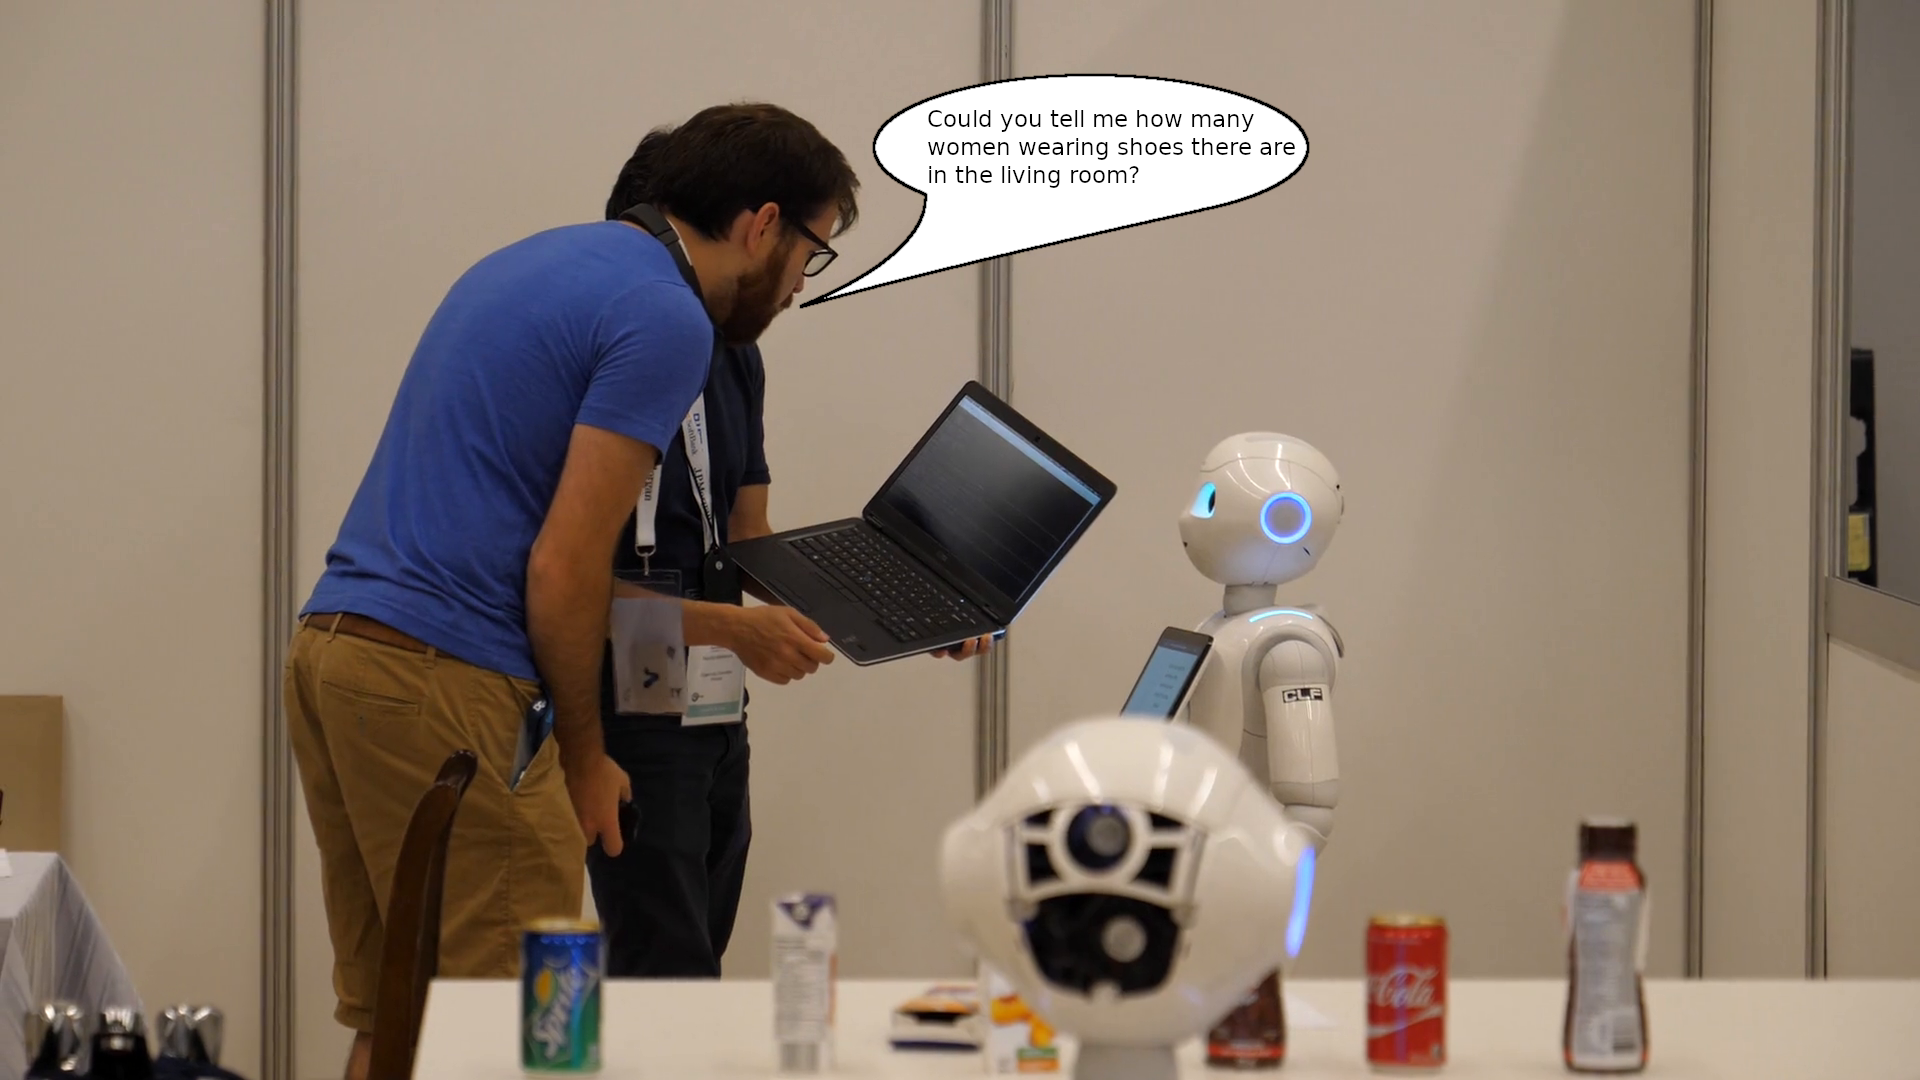
\includegraphics[width=.8\textwidth]{bilder/motivation/intro_1_edit.png}\\\vspace{3pt}
	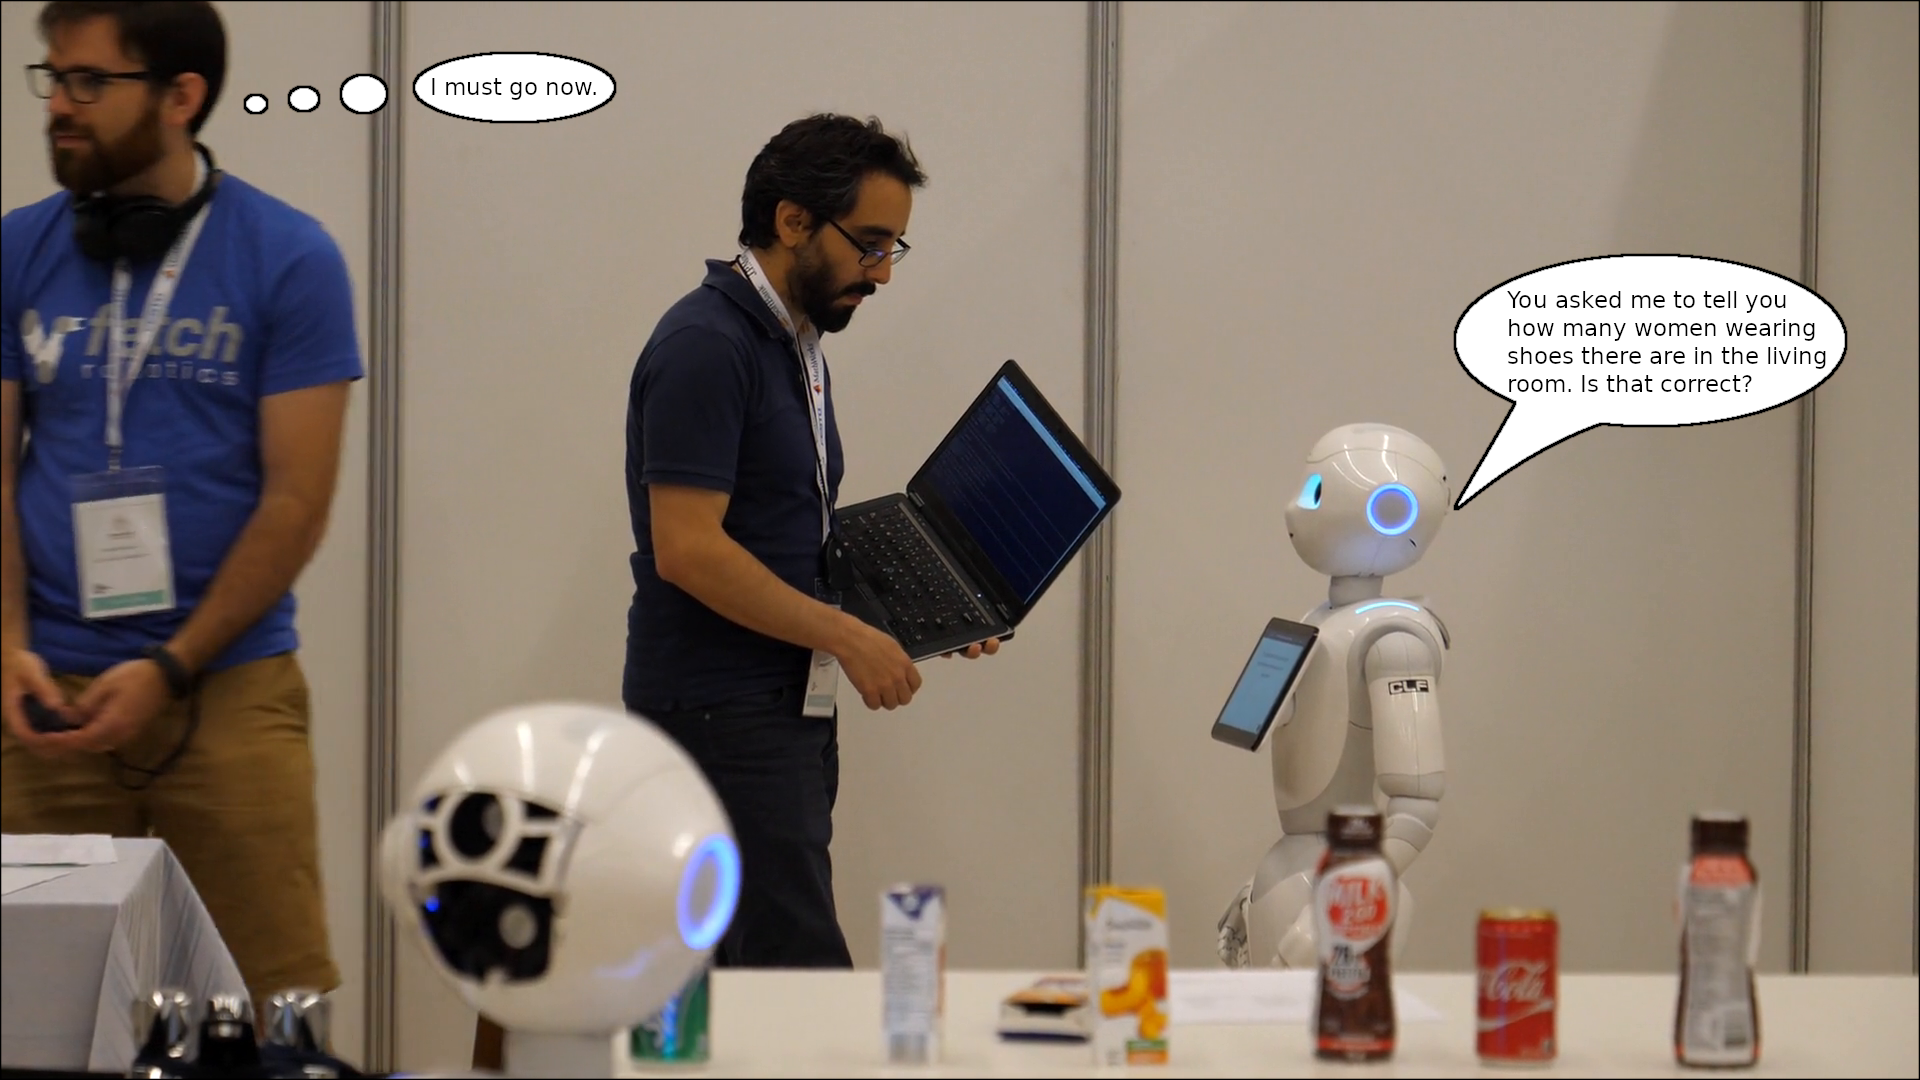
\includegraphics[width=.8\textwidth]{bilder/motivation/intro_2_edit.png}\\\vspace{3pt}
	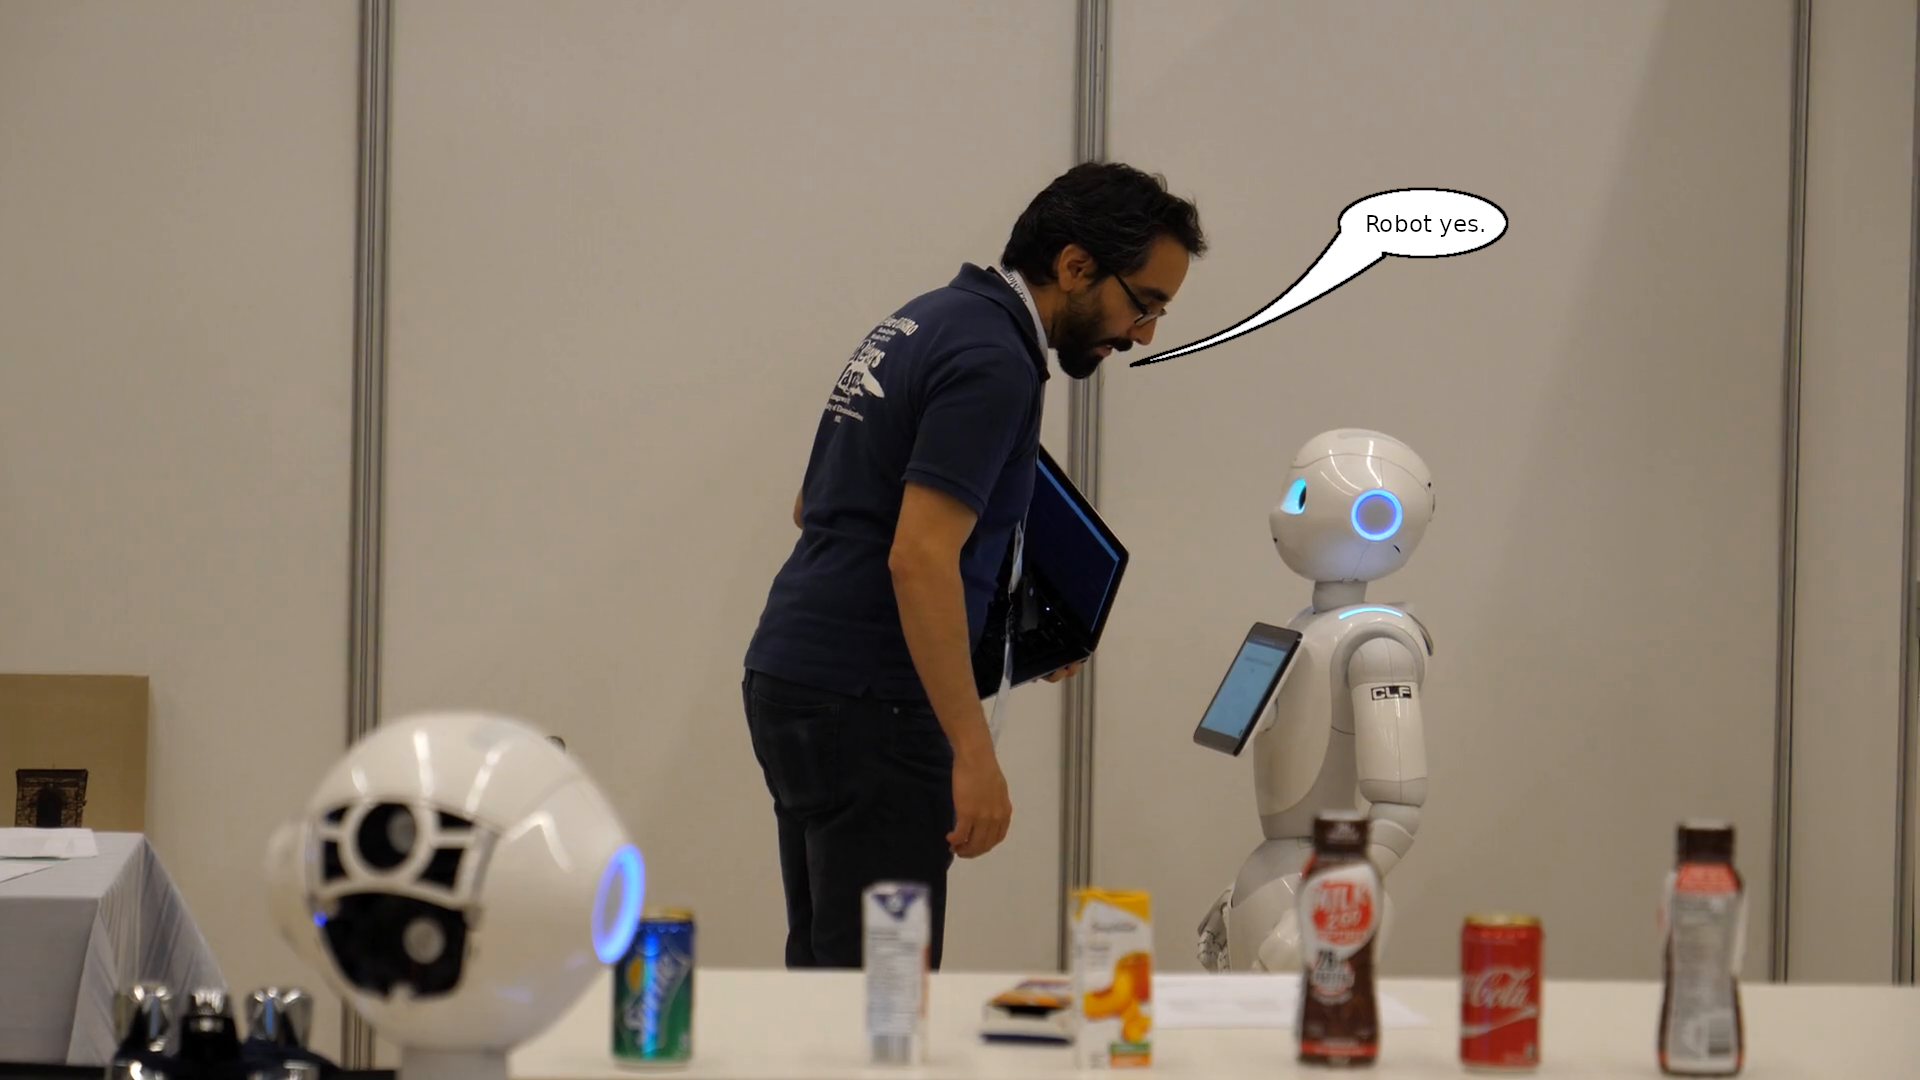
\includegraphics[width=.8\textwidth]{bilder/motivation/intro_3_edit.png}\\\vspace{3pt}
	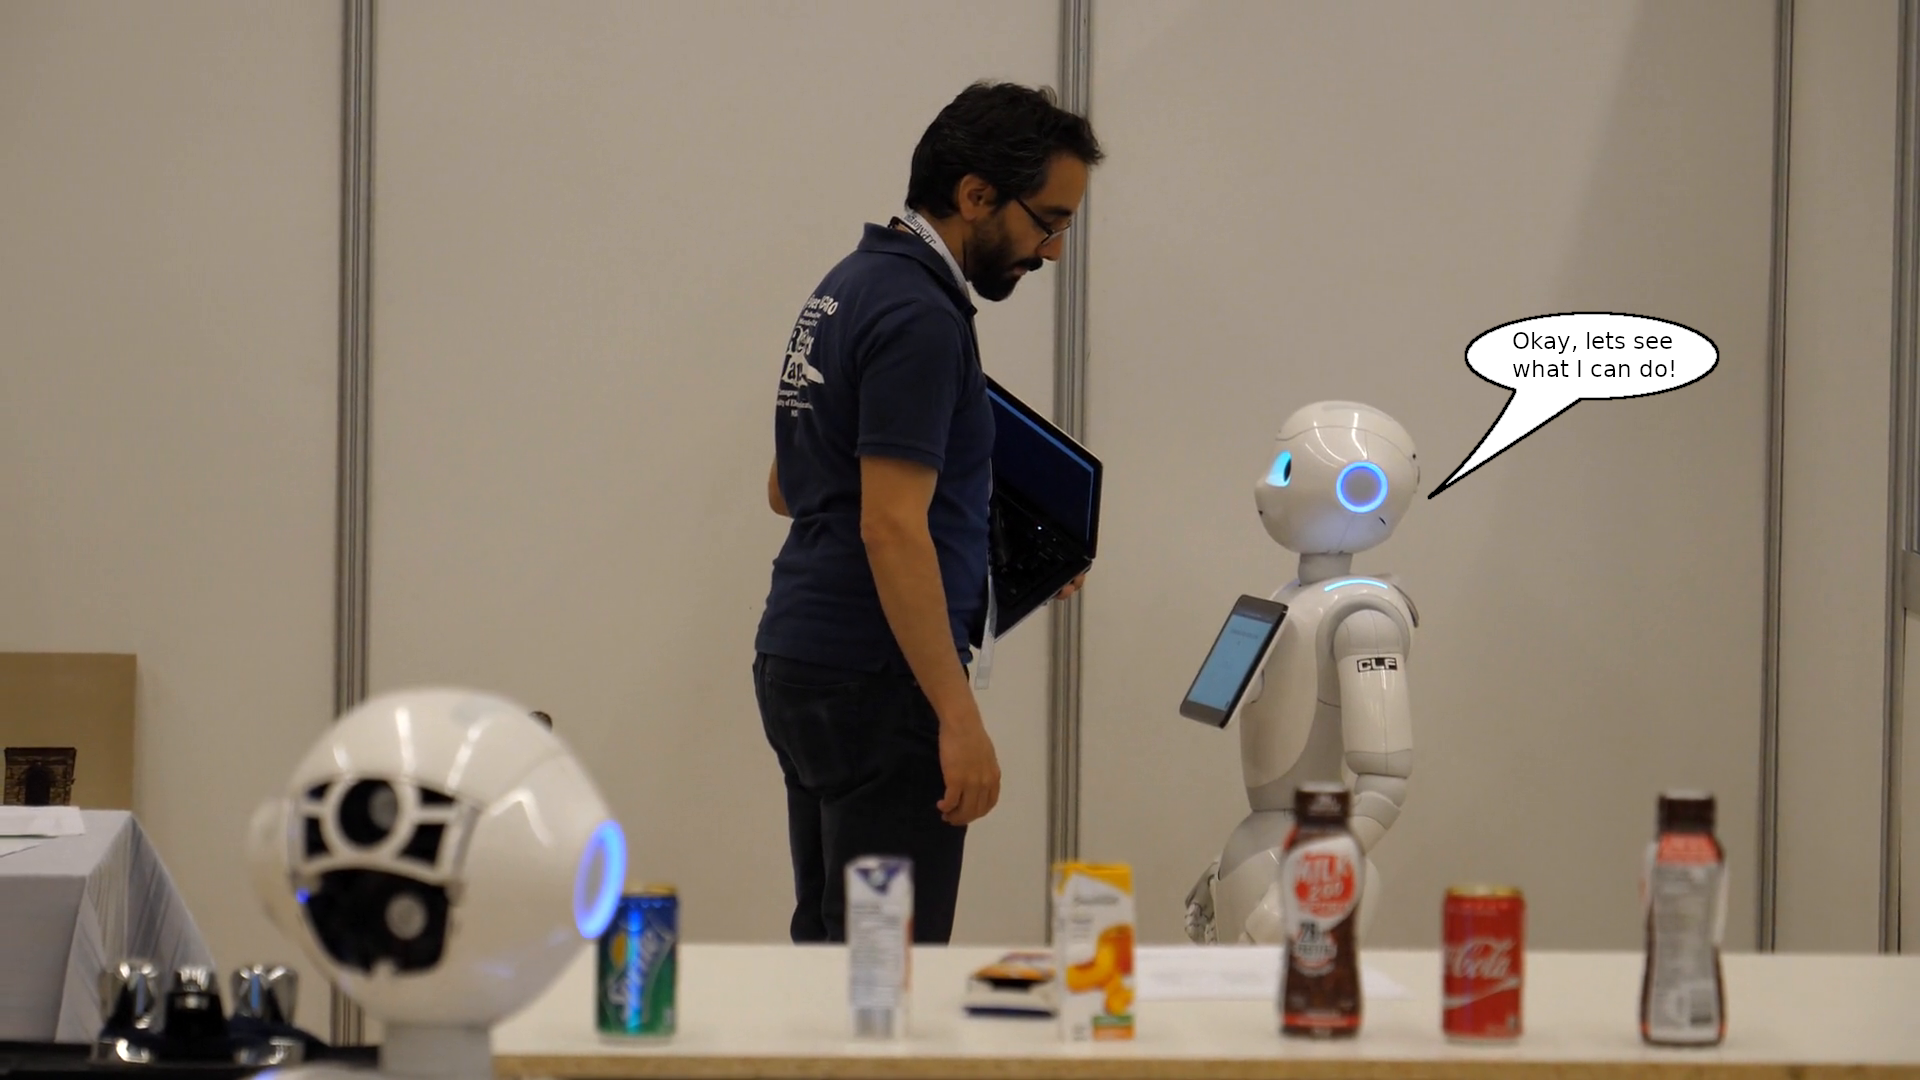
\includegraphics[width=.8\textwidth]{bilder/motivation/intro_4_edit.png}\\\vspace{3pt}
	
	\caption{Interaction between two referees and a robot in the RoboCup@home league.
		The referee in blue abandons the robot mid interaction, which does not acknowledge this at all.}
	\label{pic:moti:imustgonow}
\end{figure}

Therefore, the shown interactions appear unnatural:
the robot does not seem to perceive the human, instead it is quite clear that it just listens for a particular combination of words.
A similar phenomenon could very publicly be observed in the recent past, when Amazons Alexa ordered a variety of objects online, after hearing commands from a  TV commercial\footnote{\url{http://archive.is/zXuJu}}.
The solution employed by Amazon to stop this from happening with its own TV commercials seems to be a purposefully altered audio signal\footnote{\url{http://archive.is/d3uVu}} instead of a more general approach.

In the context of social robotics, these kinds of behavior are not desirable since approaches to partially solve these problems can be found in current literature \cite{opdenAkker:2009:YAR:1708376.1708379}.
Voice recognition technologies which can be used to differentiate speakers are available \cite{DBLP:journals/corr/abs-1003-4083}.
Additionally, computer vision is used to search for speakers, either standalone, looking for moving lips, or in combination with sound source localization (see \ref{basics:ssl}) \cite{1048137,lookwhostalking,840663,whosaidthat}.

Suitable robot behaviors need to be created, to take all this information into account.
When creating these behaviors, one must consider how the corresponding percepts are processed.
The behavior in question must either be able to combine the information, e.g. a spoken utterance and a distinct, detected voice or receive this information in a pre-combined manner.
If the behavior handles the combination, both may not be fed into the behavior at the same time, resulting in the problem to combine them.
A number of factors have to be considered when combining these information, e.g. Information may arrive asynchronous.
For example:
while just a single, long speech utterance may be received, a number of voices can be detected, or several results of the same voice.
Results in that sense are singular perceptions of a component, e.g. a voice recognizer or an \gls{ssl} detector.
Thus results have to be combined in a manner that takes this asynchrony into account.
Additionally, results will have different calculation times, based on what component created them and thus may be temporally unaligned.
This must be considered as well, creating the need to synchronize results based on their occurrence in time.

The problems just presented are clearly out of scope for robot behaviors an thus should be handled separately, due to their complexity.
I thus declare the \textbf{main goal of this thesis} to create a \textbf{framework for the automatic generation of these synchronized audio analysis results}.

Furthermore, a number of \textbf{secondary goals} can be declared.
Naturally any approach to synchronize audio results shall not have a negative impact on these results.
This can be specified in two more concrete terms.
First and foremost, the \textbf{accuracy of the results shall not decrease} by being incorporated in the proposed solution.
Second, synchronizing the \textbf{results shall not take considerably longer to compute} than not synchronizing them.
To put this into context: waiting for a result more than twice as long can not be deemed acceptable.

%---------------------------------- modularity secnd goal

Robotics is a field of intensive current research, and in the last years a number of leaps have been made.
These include, but are no limited to OpenPose \cite{cao2018openpose}, YOLO \cite{yolov3} and DeepSpeech \cite{deepspeech}.
Modularity and the ability to include such advances without the need to completely overhaul an existing system greatly decreases the time needed to incorporate such new technologies.
In turn, research speed can benefit.
I can thus declare an additional \textbf{secondary goal} in the form of \textbf{modularity}, to increase the usability of the proposed framework.

%-----------------------------------

The rest of this thesis is structured as follows:
I will first introduce concepts and frameworks in chapter \ref{basics:start}.
Here, first latency is introduced.
Latency is of special importance since it  plays a role in the computation times and is thus of particular interest with regards to the similar secondary goal.
After this I will discuss and briefly explain the concepts of \gls{asr}, \gls{ssl} and beamforming, as these can yield results of interest or be used to enhance audio signals, are partially incorporated in the later evaluation and will later present a number of challenges for the design of the proposed framework.
Finally I will explain \gls{ros}, a middleware used in the later proposed framework.

Thereafter I will present related work in chapter \ref{related:frameworks}, which will be divided in three parts.
First, a brief overview of a framework which focuses on \gls{ssl} and beamforming will be given.
Then I will discuss several fusion and synchronization approaches in preparation for my approach.
Lastly, an overview of current and former teams of the RoboCup@Home league, a prominent will be given, with special focus on their speech understanding and data fusion approaches.

After this I will present my solution in chapter \ref{main:main}.
Based on the goals formulated above and fusion approaches discussed in chapter \ref{related:fusion}, and in consideration of the concepts of latency and beamforming discussed in chapter \ref{basics:latency}, I will then present my approach for synchronization and fusion of speech analysis data.
This solution is a framework comprised of a library and a master component, the Orchestrator.
This chapter will close with an overview of the components developed over the course of this thesis.

I will then proceed to evaluate my proposed solution in chapter \ref{eval} based on two experiments.
The first experiment is conducted with the help of a data set, and is intended to evaluate the performance of the developed framework with regards to computation time.
The second experiment is heavily inspired by the ''Speech and Person Recognition'' Task of RoboCup@Home \cite{rulebook_2018}.
It is intended to evaluate the accuracy of the proposed framework in comparison to a pre-existing solution.
Both experiments will be able to show the main goal of this thesis to be achieved.
The data set experiment in particular will show the requested modularity.

Lastly I will summarize my findings and point out possible future work in chapter \ref{conclusion}.
The central point of this chapter is that due to the findings of chapter \ref{eval}, more and better components can be developed and the next step can be taken, i.e. behaviors equipped to handle situations such as those seen in figure \ref{pic:moti:imustgonow} by utilizing synchronized data can be created.

%In the appendix, I will detail the source code repositories as well as build and start instructions for the acrewed components.
%!TEX root = thesis.tex

\chapter{Related Work}

In this chapter a number of related projects and research findings will be presented and discussed. 
Several directions will be explored, i.e. an existing audio framework to transport audio \& create audio processing pipelines and different approaches to fusion of information.
Lastly RoboCup@Home, a competition between domestic robots with a strong research focus will be discussed, and several RoboCup@Home teams will be looked into with respect to their synchronization and fusion methods.

%!TEX root = ../../thesis.tex

\section{HARK}
\label{related:frameworks}
In this part \gls{hark} \cite{Nakadai_2017jrm} will be discussed, a modular framework with explicit focus on integrating beamforming and speech recognition solutions, developed by a team of researchers centered around Kyoto University.
Its goal is to provide an all in one solution for audition in robots specifically.
\gls{hark} is modular as it provides several algorithms (so called nodes) for each processing step.
These are centered around \gls{ssl}, beamforming, filtering, and feature extraction nodes.
\gls{hark} does not directly incorporate \gls{asr} solutions, but instead opts to extract audio features and send them via network to dedicated programs.
These are thusly not under its direct control.
It does not directly support other kinds of audio analysis, such as emotion-, voice-, or gender-recognition.
Nevertheless, one could develop these kinds of nodes to work with audio received via network and thus ''trick'' \gls{hark} to incorporate these nodes.
Naturally, it thus does not support the synchronization of results of any such components.
All the more, it does not support the synchronization of \gls{ssl} and \gls{asr} results, as results of \gls{asr} nodes lie outside its control.

\gls{hark} will take care of transporting audio data in between processing steps, but mostly transfers them in a frequency based representation, not as raw audio data.
This results in quite stripped down nodes, as it reduces the number of fast Fourier transforms needed to flat one instead of one per node relying on them.
Nodes which rely on raw audio however, must either manually restore the signal or use a specially developed node for this task.
Both variants results in a degrading signal however.

%-----------------------------------------------------------------------

%!TEX root = ../thesis.tex

\section{Fusion}
%!TEX root = ../../thesis.tex

\section{RoboCup@Home}
\label{related:robocup}
The RoboCup was founded in 1996 as an annual soccer competition for robots with the goal to beat the human world champions by 2050 (todo cite https://www.robocup.org/objective).
Over the years, RoboCup split into several leagues and expanded into other disciplines as well, such as the Rescue Robot league or the RoboCup@Work league.

RoboCup@Home (todo cite http://www.robocupathome.org/) is a league of the RoboCup dedicated to service robots in a domestic environment. % genauere beschreibung von @home, how is this relevant?
Therefore, human robot interaction is one of, if not the primary focus of this league.
Naturally, speech recognition systems are used as the default way to interact and communicate with the robots.
This results in the demand for robust speech recognition software.%, but also introduces problems rather unnoticed by theoretical research, such as...

One of the tasks tested in RoboCup@Home in 2017 and 2018, the ''Speech and Person Recognition'' task \cite{rulebook_2018}, is of particular interest for this work, as it mainly tests the basic speech recognition ability of the robots. 
As it was used in several RoboCup events over two years, and on dozens of robots, it is an convenient test to evaluate any speech recognition system on a robot.
Consequently, it will be used to evaluate the performance of the proposed pipeline later in chapter \ref{eval:task_start}, where the test will also be illustrated in greater detail. 

To gather information on the state of the art with regards to synchronization of sensor results and speech results in particular, I will provide an overview of established RoboCup@Home teams, which published information on that matter.
However, this information is relatively sparse in team description papers and on the teams websites, so some additional information was gathered by contacting the teams directly.

\subsection{SPQReL}
The SPQReL team from Sapienza University of Rome and the University of Lincoln use several fusion approaches. (todo cite)
Visual person perceptions were matched with \gls{ssl} results, based on their respective angular difference, and could thus be tagged as speaking.
Spoken sentences could then be mapped to speaking persons (according to email).
They employ several speech recognizers, i.e. Google Speech API and a Nuance speech recognizer, and fuse their results with a custom speech understanding system called \textit{LU4R} (todo cite), which is able to prioritize results based on expected domain specific terms. 
As such, this approach fits into the category of decision level techniques, as discussed in section \ref{related:fusion}.

\subsection{RoboFEI}
The RoboFEI team from Centro Universitário FEI in Sao Paolo (TODO cite) uses a specific microphone configuration to handle problems caused by moving sound source localization microphones.
Their robot's head is attached to a rotating pipe, which enables it to spin around its axis, while the robot's microphone array is attached to a static shaft running through that pipe which keeps it still.
As such, the position and movement of the robot's head are not relevant for sound source localization results and beamforming, and can as such be ignored.
Nevertheless, the robots own position and movement needs to be taken into account when performing \gls{ssl}, as is the case for all mobile robots.

\subsection{Tech United}
The Tech United team from the Eindhoven University of Technology provides some information about their speech recognition system.
In 2018, they generated \gls{ssl} information independently from their speech recognition.(TODO cite 2018 tdp)
They did not fuse these information however, instead opting to separately process them. %(mail)


\subsection{Walking Machine}
The Walking Machine team from École de Technologie Supérieure in Montreal (TODO cite) uses an solution, ODAS (TODO cite), which would enable them to perform \gls{ssl} and beamforming in one component, thus providing an enhanced audio signal.
However, they appear to only use its \gls{ssl} capabilities at this time.


\subsection{Kamerider}
The Kamerider team from Nankai University, China provides some information on the components they use for speech recognition and SSL (TODO cite).
They use Gstreamer to segment audio, which is then being processed by \gls{ps}.
Additionally, they use \gls{hark} for \gls{ssl}.
This way they appear to have modularized their components to a greater degree than other teams.
However, they gave no information about the interfacing of thusly acquired \gls{asr} and \gls{ssl} results.
%https://raw.githubusercontent.com/wiki/RoboCupAtHome/AtHomeCommunityWiki/files/tdp/2019-opl-kamerider_opl.pdf
 %(http://openbotics.org/kamerider/index.php?title=Main_Page)


\subsection{Hibikino Musashi}
%https://raw.githubusercontent.com/wiki/RoboCupAtHome/AtHomeCommunityWiki/files/tdp/2019-dspl-hibikino-musashiathome.pdf
The Hibikino-Musashi team of the Kyushu Institute of Technology also uses \gls{hark}, specifically its \textit{MUSIC} algorithm for \gls{ssl}.
Additionally, they employ an \gls{asr} solution in the form of \textit{Google SpeechRec} via its web API on the Chrome web browser.
We could however find no information about how the results of those components were interfaced.

\subsection{ToBi}
The team of Bielefeld (ToBi) of Bielefeld University can be discussed in greater detail, as I am a former member of this team.
For \gls{ssl} they used a proprietary solution which came with their Pepper robot %todo cite pepper and softbanks
while they used a \gls{ps} based component for \gls{asr}, the \gls{psa}. 

\gls{asr} and \gls{ssl} results are merged on the behavior layer, but only when \gls{ssl} information are explicitly needed.
The method with which they are merged is rather simplistic.
\gls{ssl} results are temporarily stored along a timestamp, which corresponds to the time these results were gathered.
Whenever an \gls{asr} result needs to be enhanced with \gls{ssl} results, an average is calculated over the \gls{ssl} results which were recorded between two and half a second before said \gls{asr} result.
This offset is employed to mitigate the time the \gls{psa} needs to recognize an utterance and the time needed by the behavior engine. 

The \gls{psa} is an \gls{asr} component which is based on \gls{ps}. \label{related_work:psa}
It captures sound directly from a microphone via \gls{alsa}, which is then segmented, to ensure only audio containing actual speech is evaluated.
It segments audio based on a loudness threshold, which, if crossed long enough, will start a segmentation.
This segmentation is ended either if a certain time limit is exceeded or if the loudness of received audio chunks drops under a second, typically slightly lower threshold.
Audio which is thus decided to contain speech will then be fed into \gls{ps}.
After a segmentation is ended, \gls{ps} will produce a result, which is then published via a \gls{ros} message.
We will use this component in later experiments (see chapters \ref{eval:dataset} and \ref{eval:task_start}).

One of these experiments will show the \gls{psa} to require considerably less time for recognitions than these 500ms.
However, a number of factors make this a good approximation still.
First, during the RoboCup@Home event, all computations are done on the robot itself, which sports considerably weaker hardware than the machine used for our experiments.
Additionally, the grammars typically used in RoboCup@Home Tasks are considerably bigger than the grammar used in our experiments, which makes matching a given utterance to a phrase in the grammar computationally more expensive.
%!TEX root = thesis.tex
%=============================================================================


\chapter{Overview}

\begin{itemize}
	\item two main problems: synchronization and transmission/ audio format adjusting
	\item division between library and orchestrator
	\item library as abstraction layer for resampling, transmission and tool to retrieve correlated information, e.g. VAD and SSL results
	\item orchestrator as central control node to manage all participating nodes
	\item ``perspective'' from outside, interfaces into and out of the pipeline
	\item most important ros messages and why they were designed as they were (AugmentedAudio.msg and EsiafRosMsg.msg)
\end{itemize}

general design decisions regarding:

\begin{itemize}
	\item latency
	\item parallelism/ pipeline tree generation
	\item architecture (distributed vs centralized (need for orchestrator))
	\item decision for using ros as an additional middleware (and against jackaudio, gstreamer, alsa, just TCP)
	\item the need for client side selectable audio format 
\end{itemize}

interaction between library and orchestrator

\begin{itemize}
	\item interfaces the orchestrator provides for the clients
\end{itemize}
%!TEX root = thesis.tex

%=============================================================================


\chapter{Orchestrator}

- manages all participating nodes

- optimizes audio 

- handles synchronization task
%!TEX root = ../../thesis.tex

%=============================================================================


\section{Library}
\label{main:lib}
In this part of this thesis the library of the proposed framework will described, along with its tasks.
As discussed earlier, the library of the proposed framework solves a number of problems, which are either directly needed for synchronization of results or make it considerably easier.
First the reasoning for some major design decision will be laid down.
After this more technical details and explanations will follow.


% audio transmission
\label{main:lib:formats}
One of the central tasks of the library involves transmitting audio from component to component.
This includes some aspects not immediately obvious.
One of those is the audio format each component requires.
An audio format determines the structure of the audio data on a lower level.
Typically, the structure of any audio data can be described by four factors:
\begin{enumerate}
	\item Its \textit{Samplerate}, which determines the resolution of an audio signal is in time domain.
	\item Its \textit{Bitrate}, which determines the resolution of the singular data points within a audio signal.
	\item Its \textit{Endianness}, which determines the order of bytes of the singular data points within a audio signal. Litte-endian encoding puts the least significant bytes first, while big-endian encoding puts the most significant bytes first. 
	\item Its \textit{Channel Count}, which determines the number of distinct audio signals within the signal. When recording audio, the \textit{Channel Count} is generally equivalent to the number of microphones used to record the audio signal.
\end{enumerate}
Working on audio data which is present in a different format then expected will in most cases lead to unusable results, maybe even to critical segmentation faults. 

Under normal circumstances, a component will request audio in the format it requires directly, e.g. via \gls{alsa}.
However, as the library now handles all audio transmission, this is no longer feasible.
With respect to one of the secondary goals of this thesis, to provide a modular framework, every components algorithm can also not be assumed to work with a specific audio format.
This leaves us to either require each component to use a single, pre-determined audio format or resampling and converting audio signals for each component.
By handling resampling and converting of audio signals within the library, components of the resulting framework can theoretically employ any kind of algorithm they desire, without having to handle resampling and converting audio themselves.
Furthermore, by abstracting resampling and converting from the components themselves, the library can be equipped to change audio formats adaptively when new components are introduced or old components vanish from a specific configuration, in a standardized way.

Consequently, the library needs to be able to resample and convert audio between arbitrary audio formats.
We chose the \gls{soxr} library \cite{soxr,soxrbase}, to resample the audio and use a custom implementation to change its \textit{Bitrate}.
The library does not handle different \textit{Channel Counts}.
The reason for this is the absence of a sufficient default behavior.
While creating a two channel audio signal from a single channel is easily done by doubling it, how to convert a two channel signal with non-identical tracks into a three channel signal?
What about the other way round?
Should a two channel signal be interpolated from a three channel signal, or should one of the tracks be discarded?
The answers to these questions differ from case to case.
As such, it seems more wise to separate the channel mechanics into dedicated components and entrust the user with finding the best choice. 
We prepared the library to handle different \textit{Endianness}, but ultimately did not implement such a feature, as different byte order is mostly a historic phenomenon and most modern operating systems, such as Windows, MacOs and most Unix systems, use little-endian encoding.

From the perspective of the library, it can then be divided between an externally used format, which is the format in which the component provides or requests audio data to the library; and an internally used format, which is the format in which the audio is transmitted.
Both of these can be identical, but must not be.
Resampling and converting of audio signals should be minimized, so careful consideration is required when choosing the format with which to transmit audio between components.

\label{main:lib:format_chooosing}
It is however equally important where these formats are chosen, as it could be done in two ways:
Either in a distributed manner, where all existing components must communicate with each other and come to a single conclusion.
Alternatively they could be determined in a centralized manner, where a single master program will collect information about each component and then based on this information will make a decision.
This was the chosen course of action, which was motivated as follows:
The main advantage of a distributed approach is that it does not rely on an additional program, as does the centralized approach.
It does so however at a cost. 
Due to the nature of the distributed approach each component taking part must have the same information as each other, that is to say each component must have information about at least each other component.
See for example figure \ref{pic:main:lib:central_vs_dist}.
In this scenario of average complexity one can clearly see the centralized approach to introduce less overhead.
While the communication between \texttt{c\_1} and \texttt{c\_2} is straight forward within the distributed approach, the communication between \texttt{c\_2}, \texttt{c\_3}, \texttt{c\_4} and \texttt{c\_5} becomes quite convoluted.
Additionally, the way in which each format is determined must be deterministic, as each component must come to the same conclusion.
All this results in a not insignificant overhead in both computational load and inter-component communication.

However, as there is already always an additional program  employed to synchronize the results, namely the Orchestrator, the benefit of the distributed approach becomes negligible.
We thus chose to implement the centralized approach with the Orchestrator as the master component, which determines each components internally used audio format.
We will go into detail how the Orchestrator chooses these formats in the following section \ref{main:orc}.

\begin{figure}[]
	\centering
	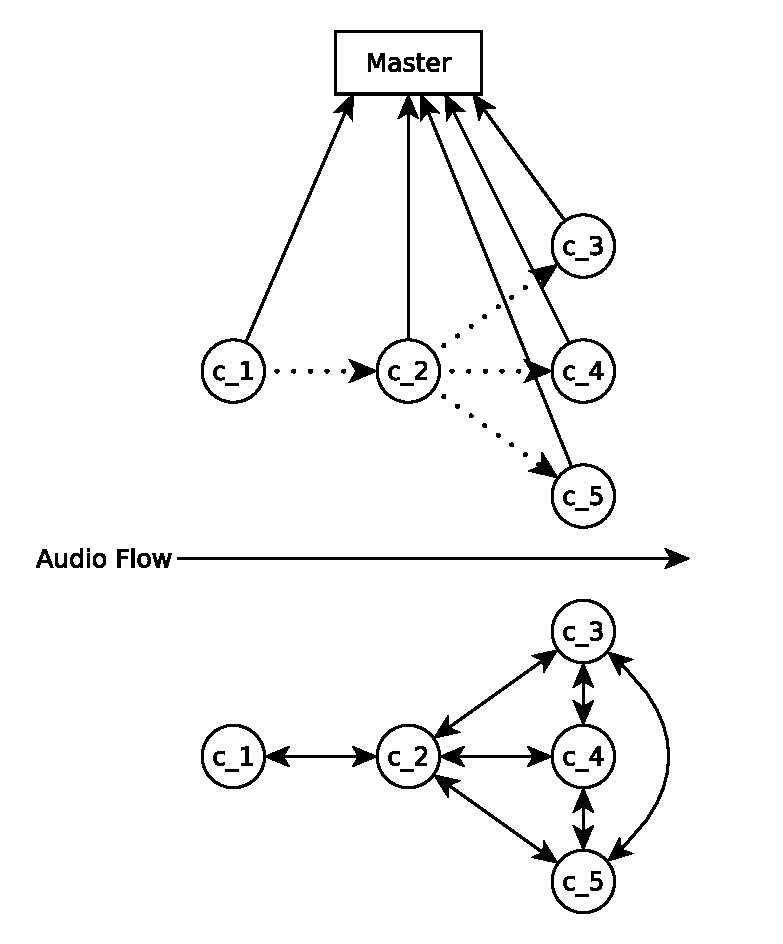
\includegraphics[width=0.66\textwidth]{diagrams/lib_central_vs_dist.pdf}
	\caption{Centralized (above) versus distributed (below) approach of determining audio formats between the components \texttt{c\_1} to \texttt{c\_5}.
		Information sending about each nodes preferred audio topic format are indicated by arrows.
		The direction of audio transmission is indicated by pointed lines above, and from left to right generally speaking.}
	\label{pic:main:lib:central_vs_dist}
\end{figure}

% python bindings
Our library was developed in C++, do to it having access to a number of very widely used and tested libraries for audio processing, such as \gls{sox} as well as its speed.
However, a number of interesting software was developed for Python, see for example libraries on which I based most of the developed components, discussed below in chapter \ref{main:components:start}.
This is what drove us to develop Python bindings for the library, using Boost Python \cite{Abrahams2003BuildingHS}.
It proved fruitful, as most the then developed components actually make use of these bindings rather then the original C++ library.
Developing the library in Python in the first place was considered, but ultimately not chosen because of C++'s superior support with regards to sound libraries, such as \gls{sox} and \gls{soxr}.

\label{main:lib:message_types}
Another important task of the library is to provide standardized \gls{ros} messages of common results generated from raw audio.
This is realized by a number of \gls{ros} messages, dedicated to speech-, emotion-, gender-, voice-, \gls{ssl}-, and \gls{vad}- information.
These messages can be inspected in figure \ref{table:main:lib:messages}.
They generally consist of a start \& end timestamp, a probability and a string containing their actual result.
Special cases are the \textit{VADInfo} message, which lacks such a string, as it only needs to capture a timeframe, 
the \textit{SpeechInfo} message, which consists of a list of result strings and their respective probabilities, along with an duration, 
and the \textit{SSLInfo} message, which in addition to a duration fields a list of \gls{ssl} outcomes, determined by an vertical as well as horizontal angle and a distinct source ID.
In any case, these must be published by the components to similarly standardized \gls{ros}-topics, consisting of the name of the component and the type of the message.

\begin{figure}[]
	\centering
	\begin{tabular}{| l | l |}
		\hline
		\multicolumn{2}{|c|}{\textbf{Duration}} \\\hline
		start & finish \\\hline
	\end{tabular}\\\vspace{0.3cm}
	
	\begin{tabular}{| l | l | l |}
		\hline
		
		\multicolumn{3}{|c|}{\textbf{GenderInfo}} \\ \hline
		gender* & probability & Duration \\\hline
	\end{tabular}\\\vspace{0.3cm}
	
	\begin{tabular}{| l | l | l |}
		\hline
		
		\multicolumn{3}{|c|}{\textbf{EmotionInfo}} \\ \hline
		emotion* & probability & Duration  \\\hline
	\end{tabular}\\\vspace{0.3cm}
	
	\begin{tabular}{| l | l | l |}
		\hline
		
		\multicolumn{3}{|c|}{\textbf{VoiceIdInfo}} \\ \hline
		voiceId* & probability & Duration  \\\hline
	\end{tabular}\\\vspace{0.3cm}
	
	\begin{tabular}{| l | l |}
		\hline
		
		\multicolumn{2}{|c|}{\textbf{VADInfo}} \\ \hline
		probability & Duration  \\\hline
	\end{tabular}\\\vspace{0.3cm}
	
	\begin{tabular}{| l | l | l |}
		\hline
		
		\multicolumn{3}{|c|}{\textbf{SpeechInfo}} \\ \hline
		\multicolumn{2}{|c|}{hypotheses[]} & Duration  \\\cline{1-2}
		recognizedSpeech* & probability & \\\hline
	\end{tabular}\\\vspace{0.3cm}
	
	\begin{tabular}{| l | l | l | l|}
		\hline
		
		\multicolumn{4}{|c|}{\textbf{SSLInfo}} \\ \hline
		\multicolumn{3}{|c|}{directions[]} & Duration  \\\cline{1-3}
		sourceId* & angleVertical & angleHorizontal & \\\hline
	\end{tabular}\\\vspace{0.3cm}
	
	\begin{tabular}{| l | l | l |}
		\hline
		
		\multicolumn{3}{|c|}{\textbf{EsiafRosMsg}} \\ \hline
		GenderInfo[]	& EmotionInfo[]	& VoiceIdInfo[]	\\\hline
		VADInfo[]	& SpeechInfo[]	& SSLInfo[] \\\hline
	\end{tabular}
	\caption{A list of all available result messages and their composition.
		All entries indicated with a star are of type string and generally used for result transmission.
		All other entries are either of a type shown here (e.g. Duration), or are floats.
		Square brackets indicate this entry to be a list of this type with unspecified length.
		The EsiafRosMsg is a special type reserved for usage by the Orchestrator, as it represents the message of synchronized results.
		}
	\label{table:main:lib:messages}
\end{figure}

%--------------------------------------------------------------------

We will now illustrate the tasks handled by the library by means of typical actions taken by an example component in its life-cycle.
Our example will be that of a typical \gls{vad} component.
As \gls{ros}is used as an underlying middleware, components within the proposed framework must also use \gls{ros} for a number of tasks.
Thus it is necessary for the component to first initialize \gls{ros}.
Following this, the proposed library will need to be initialized, which is done by first creating a handle.
This handle keeps track of all relevant information the proposed library needs.

Our example component may then declare its intention to output or request audio.
In the example, the \gls{vad} component will first declare its intend to output audio and then to require audio.
However, the library does not put a limit as to how many in- \& outputs a component can request, so an identifier is needed.
The same identifier will later internally used to generate the \gls{ros} topics with which the actual audio will be transmitted.
So it also serves to map the audio between components.%todo formulierung
If the \gls{vad} component would use the input topic \texttt{''vad\_input''}, then a microphone component would be needed to output on the same topic, so that the audio could be correctly transmitted.
Also needed to request an audio in- or output is the format in which the audio should arrive or will be given to the library respectively.

When declaring the output of audio, there are no further requirements.
When requesting audio however, the component must present the library with a callback function.
This function will later be invoked when audio was send to the component.

\label{main:lib:augmented_audio_msg}
Later, when the component is finished initializing the library and is working, % fomulierung
the component will want to actually receive and output audio.
To output audio, it will need to provide the raw audio signal in the format that it chose previously and its timestamps along with the topic on which this audio shall be transmitted.
The library will then convert this raw audio signal and its corresponding timestamps to a \textit{Augmented Audio Message}, as seen in figure \ref{pic:main:lib:augmented_audio}.
The information contained in these messages can be divided into three categories:
\begin{enumerate}
	\item Transmission information
	\item Synchronization information
	\item Meta information
\end{enumerate}
The transmission information consists of the audio signal to be transmitted as well as an message ID.
This ID is generated by the library on the transmitting side and is consecutive.
\gls{ros} as a middleware does not ensure messages to arrive at a node in the same order they were sent.
Thus, by adding an ID to each message, the receiving side of the library can later rearrange the order of arrival, should messages arrive out-of-order.
The library will also resample and convert the raw audio signal it received in the externally used format into the internally used format, if these are not identical.
Depending on the size of audio chunk this part of the message should normally be the largest.
It must be noted however, that because picking the right size of audio chunking is a non-trivial exercise (see chapter \ref{basics:latency}), the library does not give any restrictions on the size of the audio signal to be transmitted.
Even varying the size of the audio chunks between messages is allowed.  

The synchronization information is the part of the message which carries the timestamps corresponding to the audio signal.
It therefore enables components to enhance their results with accurate timestamps which in turn are later synchronized by the Orchestrator.

The last part of the message consists of optional meta information.
These meta information can be \gls{ssl} or \gls{vad} information.
As previously discussed, this information must be published by their respective nodes to the Orchestrator for synchronization purposes.
However, as a special case for \gls{ssl} and \gls{vad} components, they should also enhance the audio information with them.
The reasoning behind this is rather straight forward:
Most beamforming components will need \gls{ssl} information to work correctly.
If these information are not transmitted with the audio signal, the beamformer would need to acquire these information by itself.
After this it would then need to synchronize the \gls{ssl} information with the audio signal.
%This could most probably not be done with the help of the Orchestrator, as a beamformer enhances the audio signal for other components and the Orchestrator would aspire to fuse results by these components with the \gls{ssl} information before outputting them.
We would thus task a component of this thesis proposed framework with the very goal of this thesis.
How absurd this would be.
If these information are however included in the audio signal themselves, they are automatically fused and the beamformer can begin its work outright.
This argument works analogous with \gls{asr} components and the \gls{vad} information.

To enhance an \textit{Augmented Audio Message} with these meta information, a given component must explicitly send them to the library before outputting said \textit{Augmented Audio Message}.
To receive these information, the component must provide the library with a callback function for each.
The receiving component will have all of its callback functions be called in the opposite order.
This process can also be seen in figure \ref{pic:main:lib:ssl_vad_time}.
To come back to the example component:
Our \gls{vad} component would, upon receiving audio, first generate their \gls{vad} information, which it would then publish to the Orchestrator and simultaneously give this information to the library as meta information.
After this it would send the audio signal it received via the library, which would in turn enhance this audio with said \gls{vad} information.
The \textit{Augmented Audio Message} would then arrive in the library of e.g. an \gls{asr} component.
Before anything else, the library would first check the ID of the message.
If it was higher then expected, it would store this message and wait for more messages.
When the expected message arrives, audio signal is resampled and converted from the internally used format to the externally used format.
Then the input callback function of the component would be called with the timestamps and audio signal of the message.
This way the component can use the timestamps directly when publishing results, or just propagate them while outputting audio.
Subsequently the library would call first possible \gls{ssl} and then \gls{vad} meta information callback functions.
Thus it is guaranteed that all audio was processed before information about an ending utterance is given to the component. 
After all callback functions for a given message are called, the library will check for previously but out-of-order received messages and would process them in the same way.



%##########################################

\begin{figure}[]
	\centering
	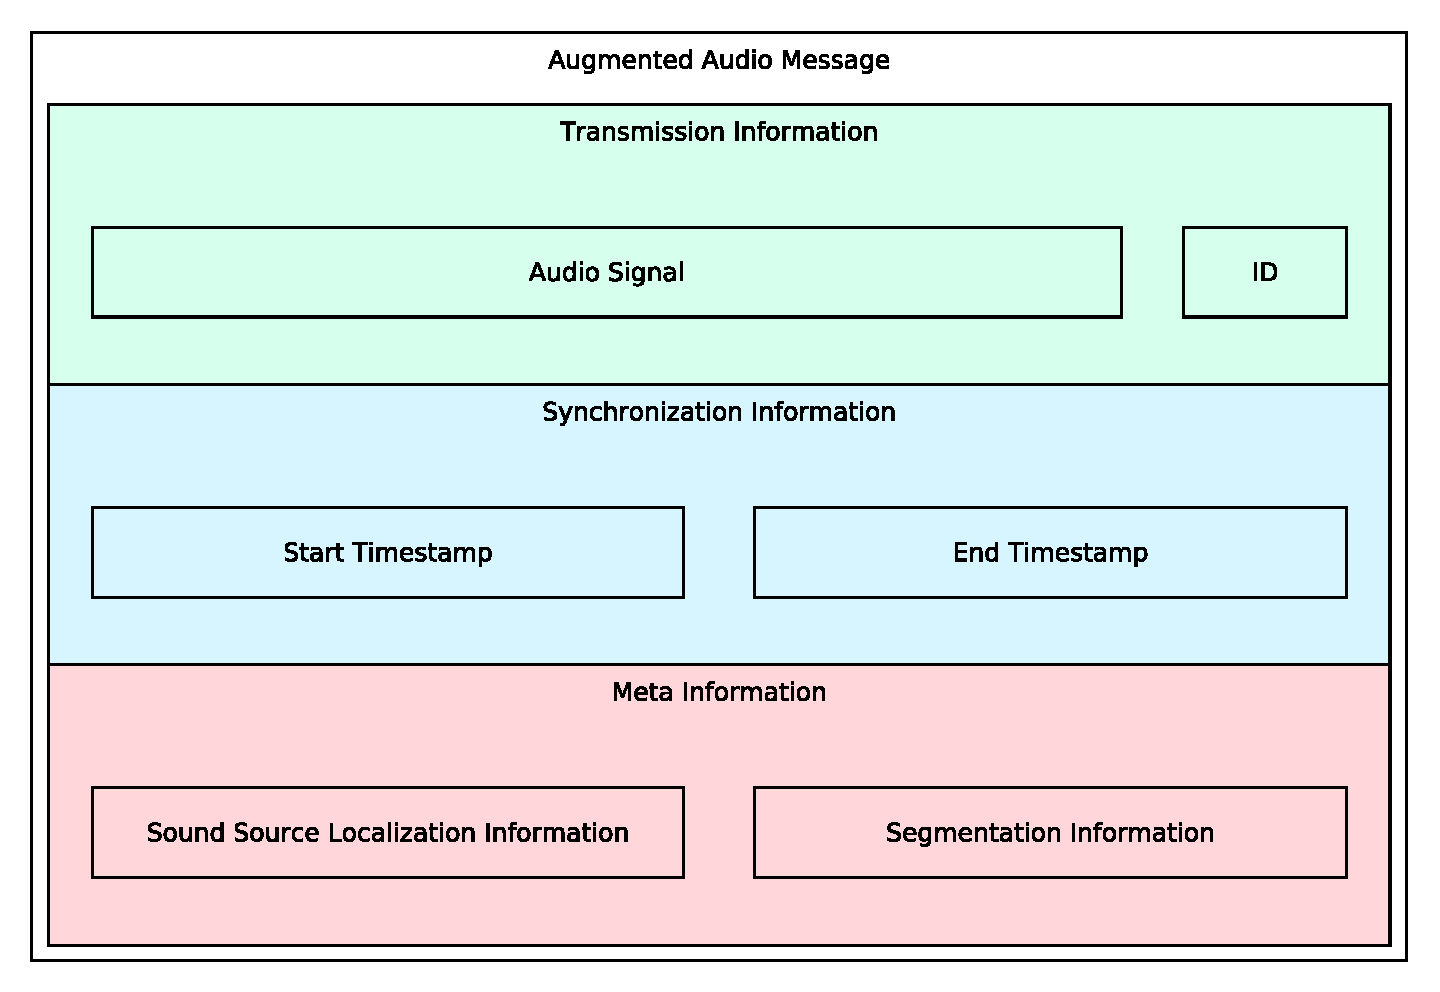
\includegraphics[width=\textwidth]{bilder/rosmsg/augmented_audio.pdf}
	\caption{Composition of Augmented Audio Messages.
		The message can be divided into three parts:
		Transmission information in green, synchronization information in blue, and Meta information in red.}
	\label{pic:main:lib:augmented_audio}
\end{figure}

\begin{figure}[]
	\centering
	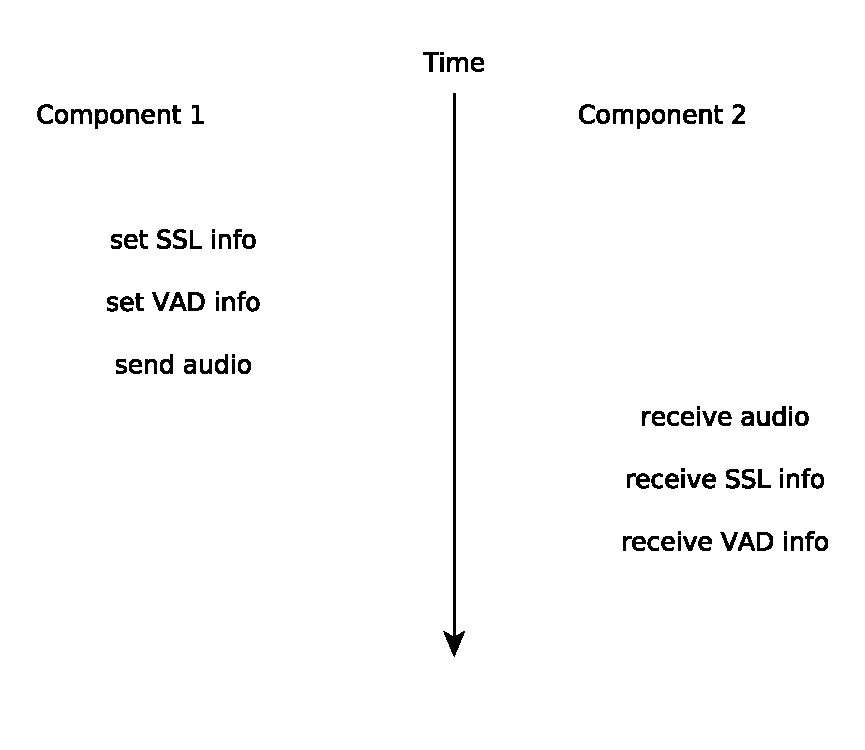
\includegraphics[width=\textwidth]{diagrams/lib_ssl_vad_time.pdf}
	\caption{Timeline of two components sending and receiving \textit{Augmented Audio Messages}.
		One can see the meta information of \gls{ssl} and \gls{vad} to be set before sending the corresponding audio, but being received after it.}
	\label{pic:main:lib:ssl_vad_time}
\end{figure}

After the declarations of audio in- \& and outputs are done, the component will signal the library to start.
Up until this point, no actual communication between the component and the Orchestrator has happened.
Now however, the library will prepare all information necessary for the Orchestrator to register the component.
Needed is the name of the component, so the Orchestrator can differentiate components from one another, as well the designation of the node, which corresponds to the task the component will perform.
We will go more into detail regarding this designation in the Orchestrator's chapter \ref{main:orc}, as it serves to easy synchronization of results.

Additionally needed are information about the in- \& output topics of audio that were previously declared.
The information about meta-information are not needed for the registration process, as they are handled internally by the library itself.
Registering the component is then done via a dedicated \gls{ros}-service, which has the library send these information
Using a \gls{ros}-service in this instance instead of a simple \gls{ros}-message has the advantage, that it can be ensured that the Orchestrator is started and ready, which may not necessarily be the case when starting the Orchestrator and components of the framework in rapid succession.

After this registration has finished, the components work may actually begin.
When the component has finished its work it may signal this to the library, or simply exit.
If the library was thusly informed, it will shut down all audio transmission.
As components cannot be expected to exit in a regulated manner in all cases, the Orchestrator must be able to handle suddenly disappearing components.
Thus there is no dedicated way to de-register a component within the library, and instead the Orchestrator handles all component shut downs.
We will focus on the Orchestrator's approach for this in the following chapter \ref{main:orc}.


%!TEX root = ../../thesis.tex

\section{Developed \& Incorporated Components}
\label{main:components:start}
In this section, components that were developed for the proposed pipeline will be discussed.
These components cover different aspects of speech recognition.

\marginnote{One good example would be a DeepSpeech component I developed\footnotemark. It makes use of a TensorFlow \cite{tensorflow} implementation of Baidus Deepspeech \cite{deepspeech}.}
\footnotetext{\url{https://github.com/Slothologist/DeepSpeech4Ros}}
Some initially planned and partially developed components were left out of this list, because it became clear they could not be included into this thesis in a meaningful way.
Thus development for these components was stopped or they were left out in favor of diverting time to more important parts of this thesis.


A handful of components are included in the library's repository, as they provide utility functions or are commonly used.
None of these components provide any information to the \textit{Orchestrator}, apart from registering.
These components are:
\begin{itemize}[leftmargin=1in]
	\item[\textit{Audio Grabber}] The \textit{Audio Grabber} is the most fundamental node, as it is the basis of most pipeline configurations.
	It is able to grab audio from a microphone via \gls{alsa} and feed it into the pipeline.

	\item[\textit{Audio Player}] This component is the \textit{Audio Grabbers} counterpart, as it receives audio data from the pipeline and outputs it via \gls{alsa} through a speaker.
	As such, it is mostly used for debugging purposes and to enable quick auditory microphone checks.

	\item[\textit{Channel Splitter}] As discussed in section \ref{main:lib:formats}, the proposed pipeline's library does not support mixing of channels.
	The \textit{Channel Splitter} is used to mitigate this absence by receiving a multichannel audio signal and produces a corresponding number of single channel outputs.
	One possible use case is to split a multichannel audio needed for \gls{ssl} into single channel audio usable for speech recognition, when no beamforming is desired.

	\item[\textit{Recorder}] The \textit{Recorder} is able to write audio it receives via the proposed pipeline to a file.
	Its foremost usage is to save audio it receives via the proposed pipeline to a file for later inspection or analysis.
	This can either be done for documentation purposes or, as was mostly done during development, to check if the pipeline transmitted and resampled audio correctly.
\end{itemize}
Additional components not included in the libraries repository cover the topics of:

\subsubsection{Wav Player}
\label{main:components:wav}
The \textit{Wav Player}\footnote{\url{https://github.com/Slothologist/esiaf_wav_player}} fulfills the same role as the \textit{Audio Grabber}, as it feeds audio into the pipeline.
However, it will read a given set of wav files in and output them into the pipeline.
It is capable of either producing silence in between each wav file or waiting for a time before playing the next file.
As such its predominant use case is to enable evaluations of other components with the help of data sets.

\subsubsection{Sound Source Localization}
\label{main:components:ssl}
I developed a component\footnote{\url{https://github.com/Slothologist/esiaf_doa}} which performs \gls{ssl}.
It uses the python library \texttt{pyroomacoustics} \cite{pyroomacoustics}, and specifically its SRP algorithm, though usage of all other \gls{ssl} algorithms provided by \texttt{pyroomacoustics} can be configured.
For each sound chunk the component receives via the proposed framework, it creates \gls{ssl} results and then sends them to the Orchestrator.

A slight variation of this node\footnote{\url{https://github.com/Slothologist/ma_baseline_doa}}  will be used in one of the experiments of the evaluation chapter (see \ref{eval:task_start}).
This variant will, instead of publishing results for each sound chunk it receives, store these results in a queue.
To communicate the results it provides a \gls{ros} service which allows any component to ask for results which occurred in a specified time frame.
Additionally, this variant will receive audio not from the proposed framework, but instead capture it from a microphone via \gls{alsa}.

\subsubsection{Voice Activity Detection}
\label{main:components:vad}
The \gls{vad} I developed\footnote{\url{https://github.com/Slothologist/AudioSegmenter}} is a reimplementation of a pre-existing algorithm present in the \gls{psa} (see chapter \ref{related_work:psa}).
Its segmentation is therefore virtually identical to the \gls{psa}'s.

If it detects the end of a segmentation, it will enhance the corresponding audio chunk with a \texttt{segmentation\_ended annotation}, as described in chapter \ref{main:lib:augmented_audio_msg}, before sending it.
Audio will not be transmitted to the next node(s) if it were not found to include speech.

\subsubsection{Automatic Speech Recognition}
\label{main:components:ps}
The \gls{asr} component I developed\footnote{\url{https://github.com/Slothologist/esiaf_pocketsphinx}} is a very simple wrapper around the python wrapper of \gls{ps}.
It will feed all audio it receives into \gls{ps}, which will then dynamically produce results.
These results are however only used if a \gls{vad} signals the end of a segment.
As such, this \gls{ps} component requires a \gls{vad} to work.
Whenever a result is produced, it is sent to the Orchestrator via published \gls{ros} message (see chapter \ref{main:lib:message_types}).

\subsubsection{Emotion Recognition}
\label{main:components:emotion}
The emotion recognition component I developed\footnote{\url{https://github.com/Slothologist/esiaf_speech_emotion_recognition}} makes use of \texttt{Speech Emotion Recognition} \cite{speech-em-rec}.
\texttt{Speech Emotion Recognition} uses a neural net to extract the emotional state of a person based on their speech.
As such, it is capable to categorize speech into three emotions: angry, happy, sad.
Additionally, speech can be categorized as neutral.
Small changes were required for it to meet all the proposed framework's expectations, so I improved it to include a probability for each result. %TODO
Each sound chunk this component acquires will be fed into \texttt{Speech Emotion Recognition} which will return an emotion and probability for each of these sound chunks.
These results are then sent to the Orchestrator for further synchronization.

\subsubsection{Gender Recognition}
\label{main:components:gender}
The gender recognition component\footnote{\url{https://github.com/Slothologist/esiaf_gender_rec}} I created is actually a somewhat new development.
It is based upon \texttt{Speech Emotion Recognition}, as it uses a nearly identical neural net and dataset.
However, I adjusted the output dimension of the neural net and reorganized its training data to classify either to male or to female, instead of the four emotions.
It also includes my changes, so its results include a probability.
I retrained the net and achieved a training accuracy of 99.63\% while maintaining a test accuracy on unseen data of 91.20\%.
Similar to the described emotion recognition component, it will produce a gender result for each sound chunk it receives along with a probability for it and send them to the Orchestrator.

It should be noted that the data set was quite small with only 339 audio samples, 188 of which by 5 female speakers , 151 from 5 male.
I suspect this being the cause for it to not achieve the level of accuracy on real world data that it achieved on the test data.
This observation is however anecdotally and was not evaluated formally.
However, I was satisfied with this solution, as it produces somewhat reasonable results.

This is especially true given the fact that it is not a part of this thesis to develop new approaches to recognition of gender, emotion or speech.
I chose this course of action with this specific component however, because an almost feasible component in the form of the described emotion recognizer was already in place and retraining of its neural net seemed to be a quick and easy way to produce a new component.
The alternative would have been to restructure and adjust a different approach, which may not have worked at all.








%!TEX root = thesis.tex
%=============================================================================


\chapter{Evaluation}

In this chapter \textit{n} tests will be presented which were used to evaluate the proposed speech recognition pipeline.

\section{Robocup Speech Recognition Test}

\section{bad wlan}
%!TEX root = thesis.tex
%=============================================================================


\chapter{Conclusion \& Future Work}
\label{conclusion}

I began this thesis with the goal to ultimately improve \gls{hri}, by providing robot behaviors with synchronized results and thus enable them to focus on perceiving humans better.
For this I created a framework which synchronizes and combines results of components of various disciplines, such as emotion and gender recognition.
Smaller, secondary goals were also formulated:
The solution was supposed to be modular, to increase its value for research.
Naturally, the solution should also perform as good as pre-existing solutions with regards to computational speed and accuracy.
This reiterated, I consider this thesis to be a mild success.

The RoboCup@Home experiment I could show my fusion approach to not only work, but to improve the accuracy of the used \gls{ssl} component in comparison to previously employed methods.
In this particular area, this thesis can be considered fully successful.
The data set experiment however is more of a mixed bag.
It inherently showed the proposed framework to be quite modular by its ability to incorporate additional components and reuse nearly all components from the RoboCup experiment.
On the other hand, it showed the proposed framework to be considerably slower then a comparable pre-existing solution.
I briefly investigated this problem and could determine the long computation time to be not be explainable by just the components and framework alone.
As such, I suspect an undiscovered bug to be he cause of this discrepancy.
Future work may thus begin by exploring this inconsistency and -if possible- eliminate it.

%--------------------

Apart from this, the logical next step would be to use the proposed framework to fed information into a robot behavior.
This way the work I presented can be properly utilized and thus improve \gls{hri} of robot, the very motivation for this thesis.
Another path for future work could start with creating more components for the proposed framework.
A number of the components I developed (see chapter \ref{main:components:start}) can not considered to be state of the art, but rather rapidly developed proofs of concept.
For productive work and actual research in the fields of speech recognition and robotics, especially multi-modal sensor fusion, as outlined in chapter \ref{related:fusion} it may prove fruitful to incorporate better performing algorithms into the proposed framework.

Another, rather unintentional feature of the proposed framework became clear when conducting the data set experiment.
The proposed framework provides a very easy way to benchmark different components against each other by providing distinct interfaces and as such a controls the environment of components to be benchmarked very tightly.
This way algorithms to be benchmarked can be controllably fed audio and their impact upon other components inspected.
It would for example be easily conceivable to test the word error rate of different combinations of \gls{vad} and \gls{asr} components.


\backmatter
%\printglossaries
\printbibliography[heading=bibintoc]

\appendix
%!TEX root = thesis.tex

%=============================================================================


\chapter*{Statement of authorship}

I hereby certify that this thesis has been composed by me and is based on my own work unless stated otherwise. 
No other person’s work has been used without due acknowledgment in this thesis. 
All references and verbatim extracts have been quoted, and all sources of information, including graphs and data sets, have been specifically acknowledged. 
This thesis has not been presented to an examination office in the same or a similar form yet.
\\\\\\\\
Bielefeld, \today
\\\\\\\\
Robert Feldhans

%=============================================================================
%\input{app_a}

\end{document}